\section{Introduction}

% Unfortunately, not all components of the SSDs have kept up with the scaling rate.
% The capacitor, which is adopted in enterprise-class SSDs for power-loss protection (PLP), fails to proceed at the pace. Historically, storage devices 
% have been equipped with a small size of volatile buffer in front of the persistent disk. 
% By using them as a read cache and a write buffer, they hide a long latency of the physical storage medium 
% as well as mitigating an endurance limitation of the worn-out devices. 
% However, the volatile buffer loses all data in the event of power crash. 
% To prevent a data loss or corruption by this, enterprise-class SSDs
% rely on the capacitors; it reserves energy to persist data in volatile buffer 
% in the unforeseen event of a power crash. 
% In addition, the adoption of capacitors enables an SSD to ignore the \texttt{FLUSH} command that explicitly requests all data in the volatile buffer to be made durable.
% This property increases the buffering effect in SSD significantly, leading to both less write traffic and a shorter operation latency.

% \EUNJI{Historically, storage devices 
% have been equipped with a small size of volatile buffer in front of the persistent disk. 
% By using them as a read cache and a write buffer, they hide a long latency of the physical storage medium 
% as well as mitigating an endurance limitation of the worn-out devices.}
The enterprise-class SSDs adopt the capacitor to protect data durability in case of power crash. 
This technique is called Power-Loss Protection (PLP) and it is needed because SSDs use a DRAM as an internal buffer for absorbing user writes and caching translation information (also known as mapping table). 
If they are not protected, SSDs will have not only a data loss and/or corruption but also a long recovery time to build an up-to-date  mapping table by scanning entire flash drives.
To preclude this situation, the enterprise-class SSDs rely on the capacitors that reserves energy to safely persist data of the volatile buffer in a power loss.

% In addition, the adoption of capacitors enables an SSD to ignore the \texttt{FLUSH} command that explicitly requests all data in the volatile buffer to be made durable.
% This property increases the buffering effect in SSD significantly, leading to both less write traffic and a shorter operation latency.

% The SSD-internal volatile buffer loses all data in the event of power crash. 
% To prevent a data loss or corruption by this, enterprise-class SSDs
% rely on the capacitors; it reserves energy to persist data in volatile buffer 
% in the unforeseen event of a power crash.
% In addition, the adoption of capacitors enables an SSD to ignore the \texttt{FLUSH} command that explicitly requests all data in the volatile buffer to be made durable.
% This property increases the buffering effect in SSD significantly, leading to both less write traffic and a shorter operation latency.

% To overcome this limitation without sacrificing performance, 
However, the \EUNJI{heavy} reliance on capacitors is no longer sustainable as the increase in SSD far outpaces 
the increase in capacitor density.
The SSD has increased significantly in density for the past decade. 
In 2011, a typical 2.5-inch SSD had 256GB capacity, but
%the world's first 2TB SSD was released in 2013~\cite{foremay2013}, but 
by 2018, a high-capacity SSD boasted a 30TB, expanding by 100× over the past ten years
~\cite{samsung2011, anandtech18samsung}. 
This remarkable growth of the device-capacity is thanks to the advanced scaling technologies 
such as nanoscale fabrication~\cite{busche2014design} and multi-layer stacking~\cite{9365809}. 
Al(aluminum) and Ta(tantalum)-electrolytic capacitors used in SSDs 
have increased in density by tenfold from 1960 to 2005. 
This is approximately 50x slower than the SSD density increase rate.
Given that the internal buffer size increases in proportion to the storage capacity,
the slow scaling of capacitors will eventually limit the amount of DRAM that can be used in an SSD. 
This, in turn, will also limit the storage capacity as the size of DRAM and aggregate flash capacity proportionally scale~\cite{samsung_ratio, ni2017hash}. 

\iffalse
the density gap between capacitance and memory technologies 
imposes an intrinsic limitation on the current architecture wherein 
the entire buffer is fully protected by capacitors. 
\fi
% \begin{figure}[t]
%     \centering{}
%     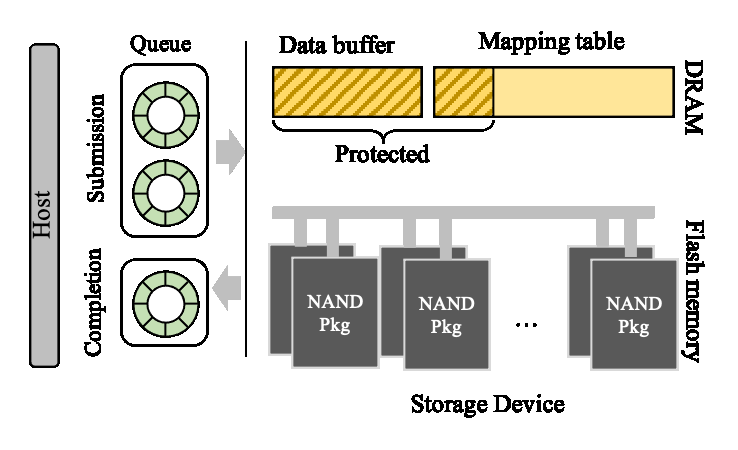
\includegraphics[width=0.4\textwidth]{figure/dawid_ssd_archi.eps}
%     %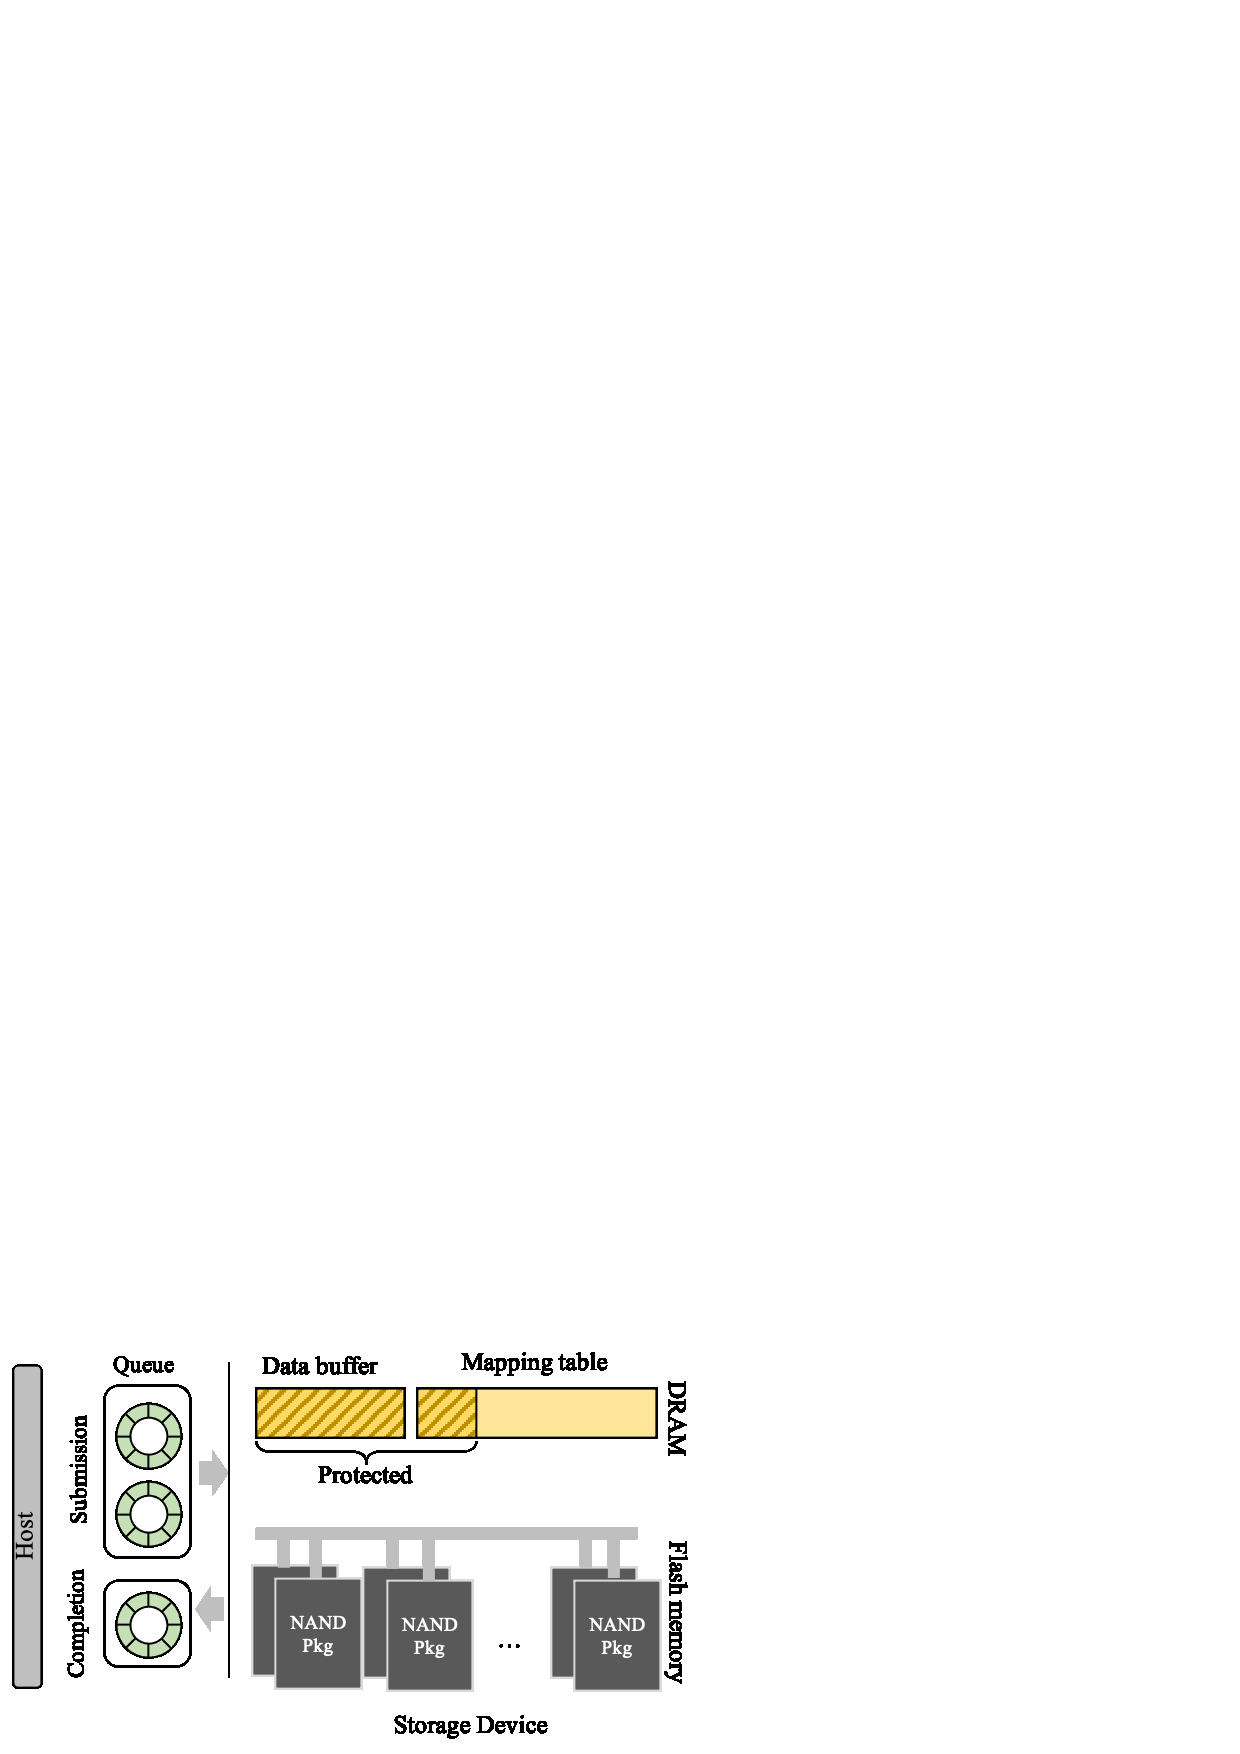
\includegraphics[width=0.4\textwidth]{figure/dawid_ssd_archi.png}
%     \caption{\textbf{SSD architecture with \ours{} buffer.}}
%     \label{fig_dawid_archi}
% \end{figure}
% \EUNJI{to scale ...}

% This paper presents a device-internal buffer architecture called \ours{}
% for the SSDs under capacitance constraints. \ours{} only XXX. 
This paper presents \ours{}, a novel SSD-internal DRAM management scheme 
that allows the SSD capacity to scale beyond the slow growth of capacitors. 
SSD-internal DRAM is used for 
(1) caching translation information (also known as mapping table) and (2) buffering user writes. 
In typical SSD designs, most of the capacitance is used for protecting the mapping table (to keep as many translation entries in DRAM) 
and the buffer for user writes is kept at a minimal (just enough to hide the flash program latency)~\cite{KangLMKO14sigmod}. 
As an example, Samsung PM1643 30.72TB and PM1633a 15.36TB house 40GB and 16GB DRAM, respectively~\cite{anandtech18samsung}. 
(typically 0.1\% of storage capacity~\cite{samsung_ratio, ni2017hash})

However, in our design, we take a radically different approach. 
We buffer more user writes so that mapping entry eviction becomes more efficient by aggregating dirty updates. 
This substantially reduces the amount of mapping table-related write traffic, and in turn, improves the overall performance under capacitance constraints. 


\textcolor{red}{
The data maintained in the buffer can be classified into two types: the actual user data and 
the metadata for SSD management (i.e, mapping table). 
When the buffer is partially protected, the number of dirty pages is limited to 
the maximum amount of data that the on-board capacitance can protect. 
If the number of dirty pages goes beyond the limit, changes should be flushed to the flash memory immediately
to meet the durability constraint for SSDs. 
}
